% ****** Start of file apssamp.tex ******
%
%   This file is part of the APS files in the REVTeX 4.2 distribution.
%   Version 4.2a of REVTeX, December 2014
%
%   Copyright (c) 2014 The American Physical Society.
%
%   See the REVTeX 4 README file for restrictions and more information.
%
% TeX'ing this file requires that you have AMS-LaTeX 2.0 installed
% as well as the rest of the prerequisites for REVTeX 4.2
%
% See the REVTeX 4 README file
% It also requires running BibTeX. The commands are as follows:
%
%  1)  latex apssamp.tex
%  2)  bibtex apssamp
%  3)  latex apssamp.tex
%  4)  latex apssamp.tex
%
\documentclass[%
 reprint,
%superscriptaddress,
%groupedaddress,
%unsortedaddress,
%runinaddress,
%frontmatterverbose, 
%preprint,
%preprintnumbers,
%nofootinbib,
%nobibnotes,
%bibnotes,
 amsmath,amssymb,
 aps,
%pra,
%prb,
%rmp,
%prstab,
%prstper,
%floatfix,
]{revtex4-2}
\usepackage{kotex}
\usepackage{graphicx}% Include figure files
\usepackage{dcolumn}% Align table columns on decimal point
\usepackage{bm}% bold math
%\usepackage{hyperref}% add hypertext capabilities
%\usepackage[mathlines]{lineno}% Enable numbering of text and display math
%\linenumbers\relax % Commence numbering lines

%\usepackage[showframe,%Uncomment any one of the following lines to test 
%%scale=0.7, marginratio={1:1, 2:3}, ignoreall,% default settings
%%text={7in,10in},centering,
%%margin=1.5in,
%%total={6.5in,8.75in}, top=1.2in, left=0.9in, includefoot,
%%height=10in,a5paper,hmargin={3cm,0.8in},
%]{geometry}

\begin{document}


\title{천연 색소의 추출과 무기 안료의 합성 결과보고서}

\author{서울대학교 전기정보공학부 2018-12432 박정현}
 \email{alexist@snu.ac.kr}
\date{실험일자 09.26.2023}% It is always \today, today,
             %  but any date may be explicitly specified

\begin{abstract}
본 실험에서는 면섬유를 매염제, 그리고 치자, 소목, 자초를 이용해 염색하였다. 이후에는 다른 pKa 값을 가지는 산 용액을 염색된 면섬유와 반응시켜 매염제의 역할, 그리고 염료의 분자구조에 따른 분자구조의 변화에 이에 따른 색변화를 고찰하였다. 이후에 반응하지 않는 면섬유들에 대해 논의한 후 이를 해결하기 위해 강산을 사용하고, 다른 작용기의 역할을 확인하기 위해 염기 용액을 이용해 반응하는 것을 고려하였다.
\end{abstract}

%\keywords{Suggested keywords}%Use showkeys class option if keyword
                              %display desired
\maketitle

%\tableofcontents

\section{\label{sec:level1}Assignment}
\subsection{\label{sec:level2}1}
소목의 경우 브라질레인(Brazilein)[4], 치자의 경우 크로신(Corcin)[5] 그리고 자초의 경우 시코닌(Shikonin)[6] 분자를 함유하고 있다. 각각의 분자는 구조는 아래와 같다.[4][5][6] 브라질레인, 크로신 모두 하이드록시기를 가지고 있고 비댕칭적이므로 극성을 띠어 친수성 분자가 된다. 반면에 시코닌의 경우 하이드록시기를 가지고 있긴 하지만 대칭적으로 존재하여 극성이 상쇄되어 거의 사라지게 된다. 또한 하나의 하이드록시기를 제외하면 분자의 대부분이 무극성이 되어 소수성이 된다. 알코올의 경우 친수성, 소수성 작용기가 모두 존재하므로 시코닌 분자는 알코올에 잘 용해될 수 있다. 따라서 본 실험에서 자초의 경우에는 알코올을 이용해 염료를 추출한다.\\

\begin{figure}[htbp]
	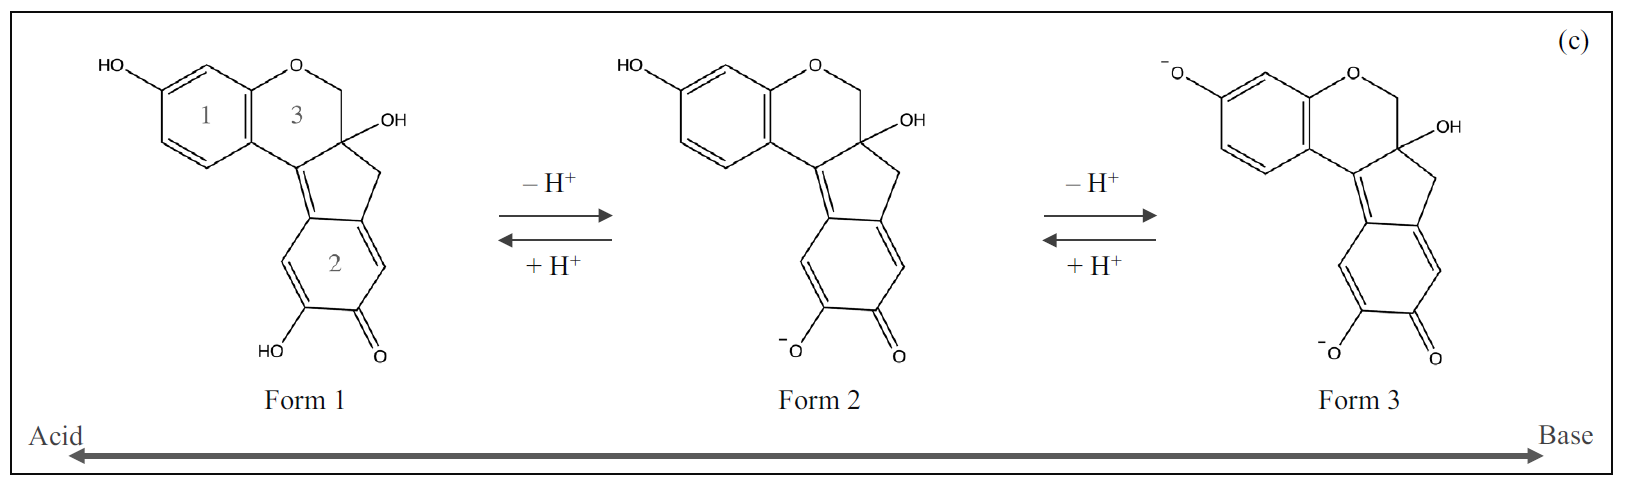
\includegraphics[width = 0.95\linewidth]{Brazilein.png}% Here is how to import EPS art
	\caption{\label{fig:Brazilein}브라질레인 분자 구조}
\end{figure}
\begin{figure}[htbp]
	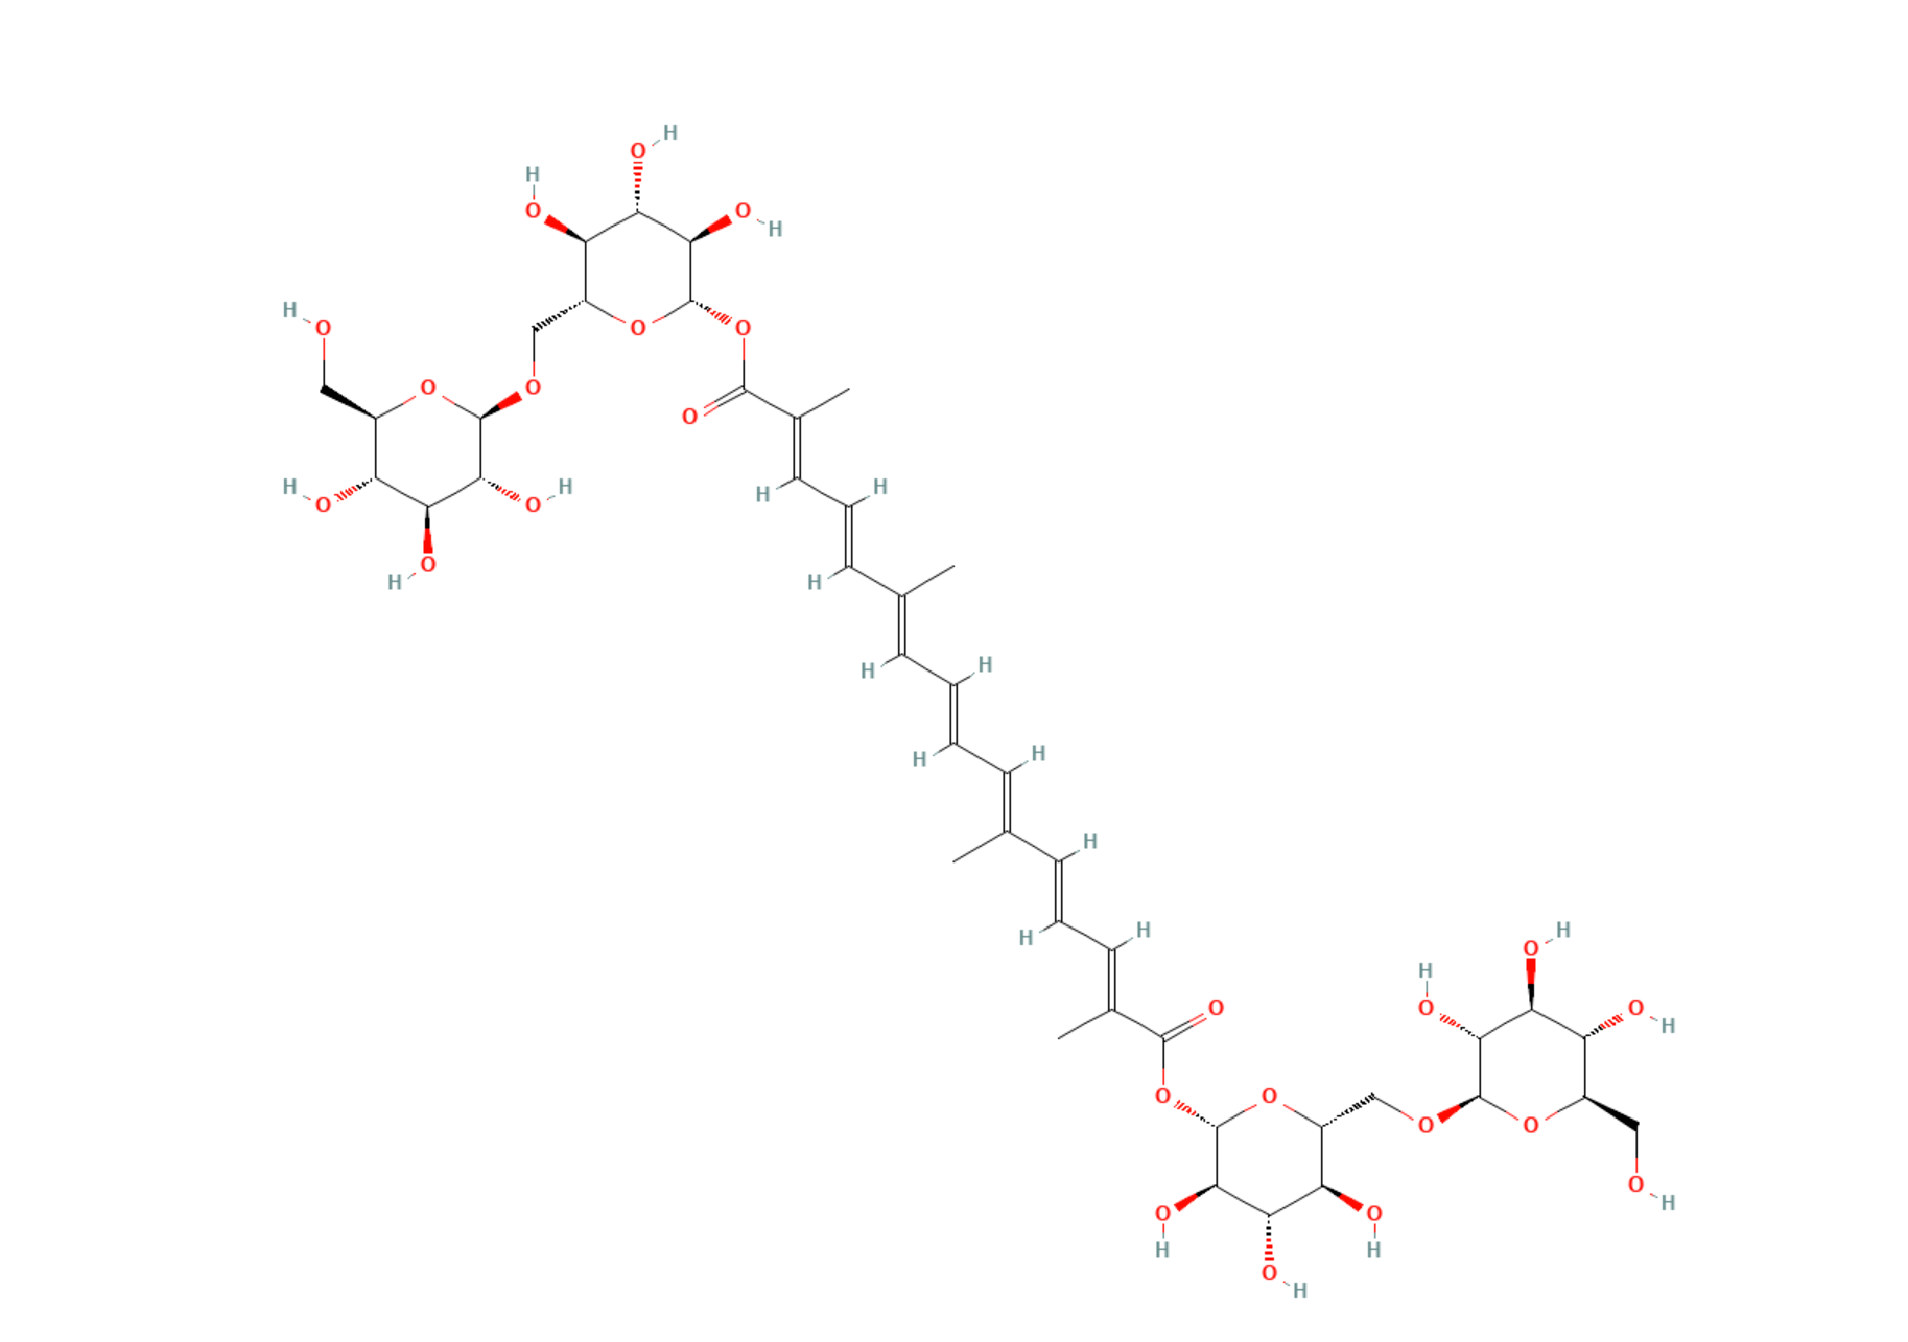
\includegraphics[width = 0.95\linewidth]{Corcin.png}% Here is how to import EPS art
	\caption{\label{fig:Corcin}크로신 분자 구조}
\end{figure}
\begin{figure}[htbp]
	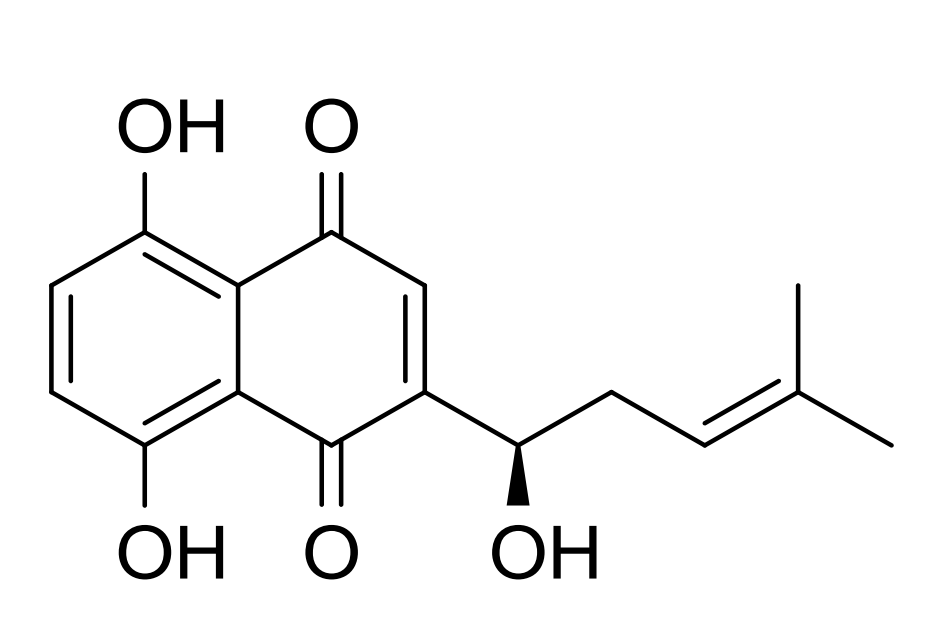
\includegraphics[width = 0.7\linewidth]{Shikonin.png}% Here is how to import EPS art
	\caption{\label{fig:Shikonin}시코닌 분자 구조}
\end{figure}

\subsection{\label{sec:level2}2}
유기 분자의 경우 $\sigma$, $\pi$ 결합이 번갈아 가며 존재하는 공명 구조가 존재한다. 이러한 공명 구조에서 흡수 방출되는 전자기파의 주파수가 가시광선에 해당하는 경우 우리의 눈에는 빛이 띠는 것으로 보이게 된다. [3] 이러한 파장은 공명하게 되는 분자의 길이에 비례하며 분자마다 공명하는 길이가 다르므로 다양한 색을 띠게 된다.\\

전이금속이 함유된 분자의 경우 음이온을 띠게 되어 양이온과 배위결합을 하여 착화합물이 형성된다. Fig.\ref{fig:d_orbital}에 나타난 전이 금속에 존재하는 d-orbital energy level이 존재한다. 양이온이 전이금속이 함유된 분자에 가까워짐에 따라 Fig.\ref{fig:energy_splitting}에 나타난 것처럼 전이금속의 d-orbital energy level을 split하게 된다. 분리된 d level에서 전자들이 광자를 흡수 방출하면서 전이하게된다. 이러한 광자가 가시광선 파장대역에 해당하면 사람들에게는 색깔이 있는 것으로 보인다.[2]
\begin{figure}[htbp]
	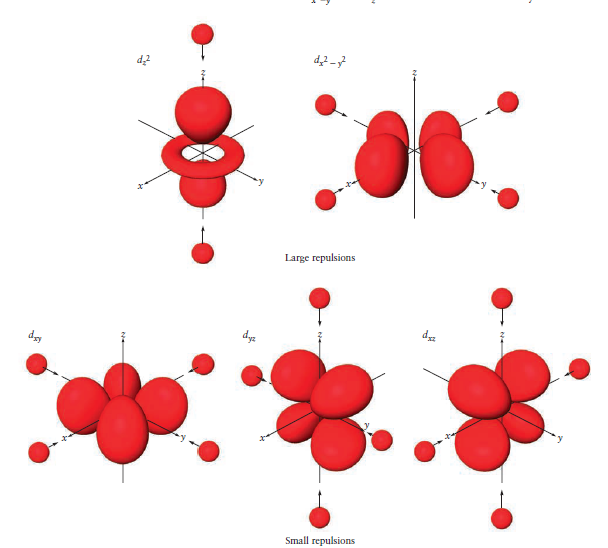
\includegraphics[width = 0.9\linewidth]{d_orbital.png}% Here is how to import EPS art
	\caption{\label{fig:d_orbital}전이금속의 d-orbital}
\end{figure}
\begin{figure}[htbp]
	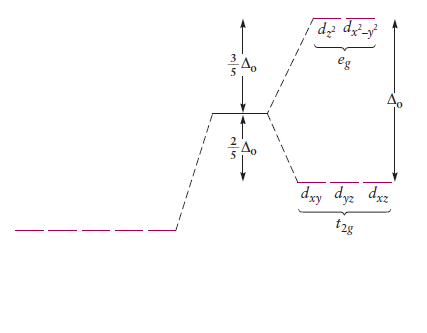
\includegraphics[width = 0.9\linewidth]{energy_splitting.png}% Here is how to import EPS art
	\caption{\label{fig:energy_splitting}배위결합에 의한 d-orbital energy split}
\end{figure}

%%%%%%%%%%%%%%%%%%%%%%%%%%%%%%%%%%%%%%%%%%%%%%%%%%%%%%%
%%%%%%%%%%%%%%%%%%%%%%%%%%%%%%%%%%%%%%%%%%%%%%%%%%%%%%%
%%%%%%%%%%%%%%%%%%%%%%%%%%%%%%%%%%%%%%%%%%%%%%%%%%%%%%%
%%%%%%%%%%%%%%%%%%%%%%%%%%%%%%%%%%%%%%%%%%%%%%%%%%%%%%%

\section{\label{sec:level1}Introduction}
\subsection{\label{sec:level2}실험 배경}
면섬유의 염색은 우리 일상의 다양한 옷이나 직물 제품에 사용되며, 그 색상의 다양성과 지속성은 많은 소비자들에게 중요하게 여겨진다. 기존에 천연염색으로 염색을 수행하였으나 시간이 지나 인공적으로 염색을 하는 방향으로 흘러갔다. 하지만 여러 환경 문제, 건강 문제 등이 논의되면서 전통적으로 천연 염료를 사용하여 면을 염색하는 방법이 대두되고 있다. 이러한 천연 염료의 분자구조와 면섬유가 어떻게 상호 작용하는지 깊이 이해하고 적용하는 것은 중요한 문제이다.\\

매염제의 역할은 염색 과정에서 중요하게 작용하는데, 매염제가 없거나 적절하지 않으면 염료가 섬유에 제대로 부착되지 않을 수 있다. 또한, 염료의 분자구조와 산-염기 반응은 색상의 변화와 밀접한 관련이 있다. 특히, 다양한 pKa 값을 가지는 산과의 반응을 통해 염료의 분자구조 변화와 그에 따른 색변화를 관찰하는 것은 면섬유 염색의 핵심 요소 중 하나이다. 본 실험에서는 면섬유의 염색 과정에서 천연 염료가 면섬유와 결합하는 방식을 이해하고 매염제의 역할, 그리고 산-염기 반응을 통한 색상 변화를 살펴보는 것을 목적으로 하였다.

\subsection{\label{sec:level2}염색}
염색을 하는 면섬유의 구조가 polyamide 중합체로 구성된 경우 면섬유에 존재하는 $NH$의 양극이 염색염료와 결합한다. 반면에 면섬유가 셀룰로우스와 같이 $OH$기가 존재하는 분자인 경우 음극이 염색염료와 수소결합을 하게 된다.[3] Figs.\ref{fig:NH3_bond}, \ref{fig:OH_bond}은 각각의 결합에 대해서 보여주고 있다. 매염제는 분자내에 존재하는 전이 금속 원자의 금속이온의 리간드에 의해 염색염료 분자와 배위결합 하여 착화합물을 형성하게 된다. 이와 같이 형성된 화학결합은 면섬유와 염색염료 사이에 강한 결합을 유지할 수 있게 만들어준다.
\begin{figure}[htbp]
	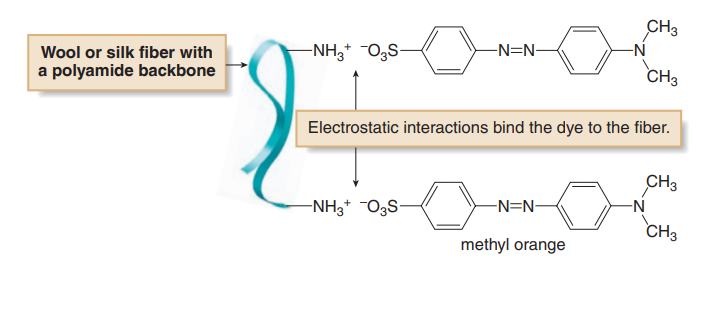
\includegraphics[width = 0.9\linewidth]{NH3_bond.png}% Here is how to import EPS art
	\caption{\label{fig:NH3_bond}염료분자와 polyamide의 결합}
\end{figure}
\begin{figure}[htbp]
	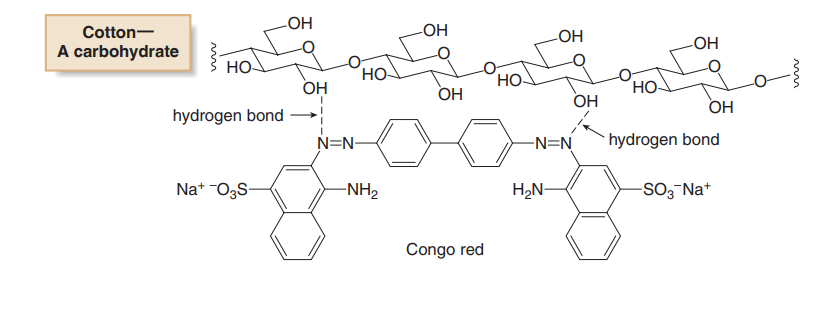
\includegraphics[width = 0.9\linewidth]{OH_bond.png}% Here is how to import EPS art
	\caption{\label{fig:OH_bond}염료분자와 carbonhydrate 분자와의 결합}
\end{figure}

\section{\label{sec:level1}Methods \& Materialsl}
$500mL$비커 1개, $100mL$비커 3개, $50mL$비커 5개, 페이퍼타월 9개, 집게, 힛플레이트, 목장갑, 받침용 페이퍼타월, $KAl(SO_{4})_{2}$ 명반, $FeSO_{4}$ 녹반, 전자저울, 약포지, 약수저, 유산지, 라텍스장갑, $50\%$에탄올, $1/20$로 희석된 아세트산, $NaHCO_{3}$ 수용액, 치자, 소목, 자초를 준비한다. 먼저 $500mL$의 비커에 물을 채우고 가열시킨다. 이후에 $50mL$비커 각각에 $1.5g$의 명반과 녹반을 담은 뒤 가열된 물을 $30mL$정도 채워주어 가열한다. 매염제가 모두 녹은 경우에는 면섬유 3장을 각각의 비커에 넣은 뒤 3분 가량 가열한 후 다른 곳에 보관한다.\\

$100mL$비커 3개에 치자, 소목, 자초를 각각 $4$, $6$, $5$개를 넣는다. 자초가 담긴 비커에는 에탄올 용액을, 치자와 소목이 담긴 비커에는 $70mL$의 물을 채운뒤 힛 플레이트에서 $200^{o}C$에서 5분 가량 가열한다. 색이 적당히 나온 경우에는 얼룩이 생기지 않도록 염료 건더기를 꺼내준다. 이후에는 매염하지 않은 면섬유를 3개의 비커에 각각 하나씩 넣은뒤 5분 가량 가열한 후 꺼내주어 물에 앃겨준다. 이후에는 천연염료를 추출한 용액을 $100mL$비커에 절반씩 분리하여 담아준다. 이후에 명반, 녹반으로 매염한 섬유들을 각각 모두 넣어준 뒤 5분 가량 가열한 후 물에 앃어서 페이퍼 타월에 올려 둔 후 기록한다. 염색된 면섬유 9개에 아세트산을 한 두 방울 떨어뜨리고, 나머지 부분에 $NaHCO_{3}$ 수용액을 한두 방울 떨어뜨린다. 이후에 흐르는 물에 씻기고 변화를 확인한 후 기록한다.

\section{\label{sec:level1}Results \& Discussion}
염색 직후, 그리고 아세트산과 $NaHCO_{3}$를 반응시킨 결과는 각각 Figs.\ref{fig:Before}, \ref{fig:After}와 같다. 명반과 녹반이 첨가된 경우 색의 변화가 발생한다. 또한 매염제 없이 소목을 이용해 염색한 경우와 명반과 소목을 이용해 염색한 경우에서 아세트산에 의한 반응을 제외하고는 다른 면섬유들은 아세트산과 $NaHCO_{3}$에 거의 반응하지 않는다.
\begin{figure}[htbp]
	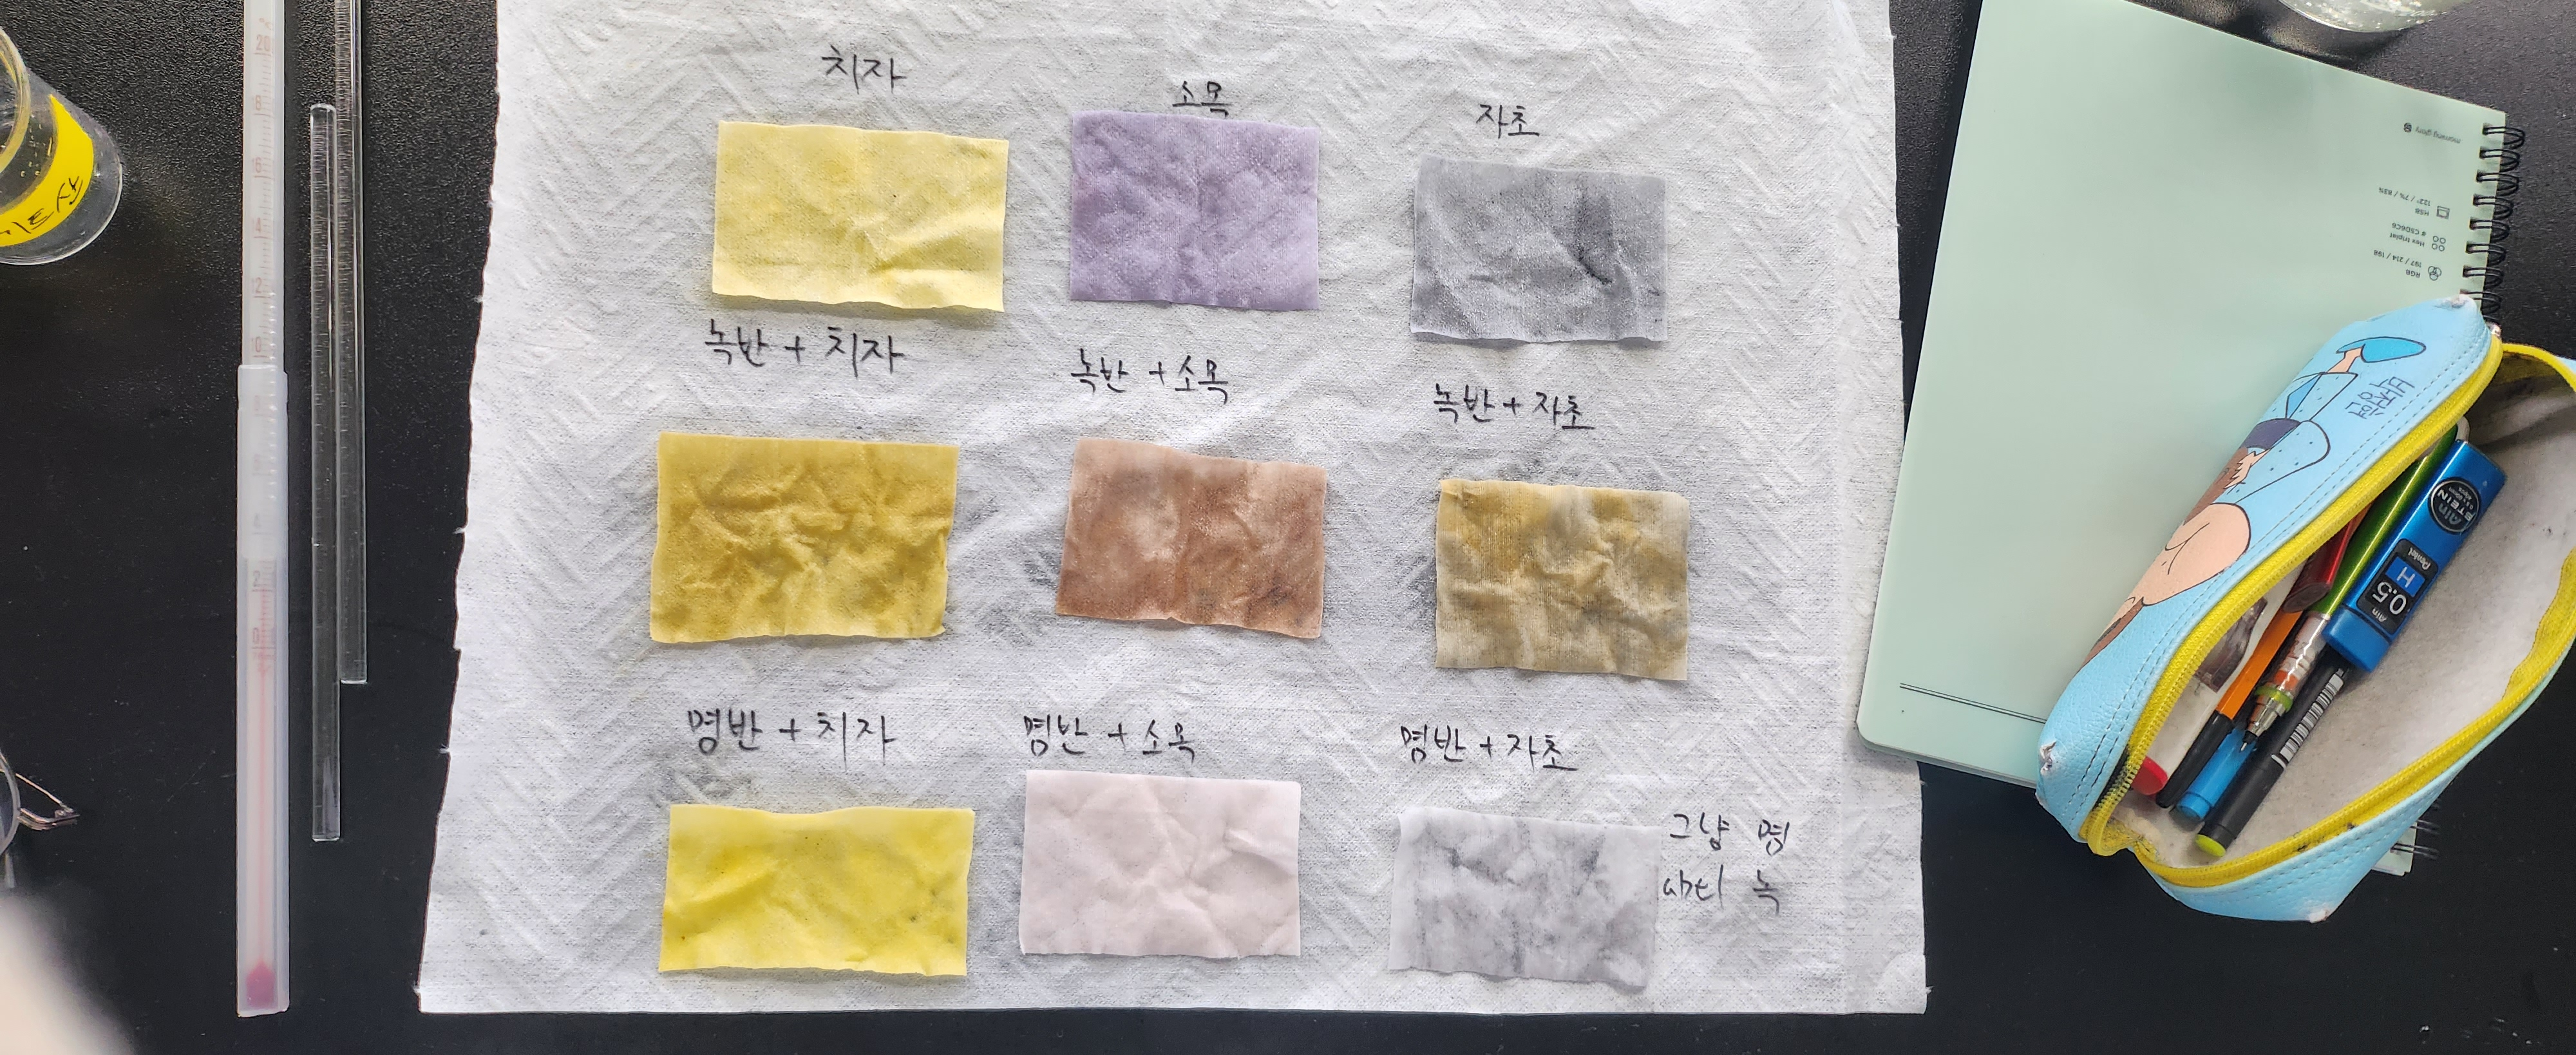
\includegraphics[width = 0.95\linewidth]{Before.png}% Here is how to import EPS art
	\caption{\label{fig:Before}염색 직후 결과}
\end{figure}
\begin{figure}[htbp]
	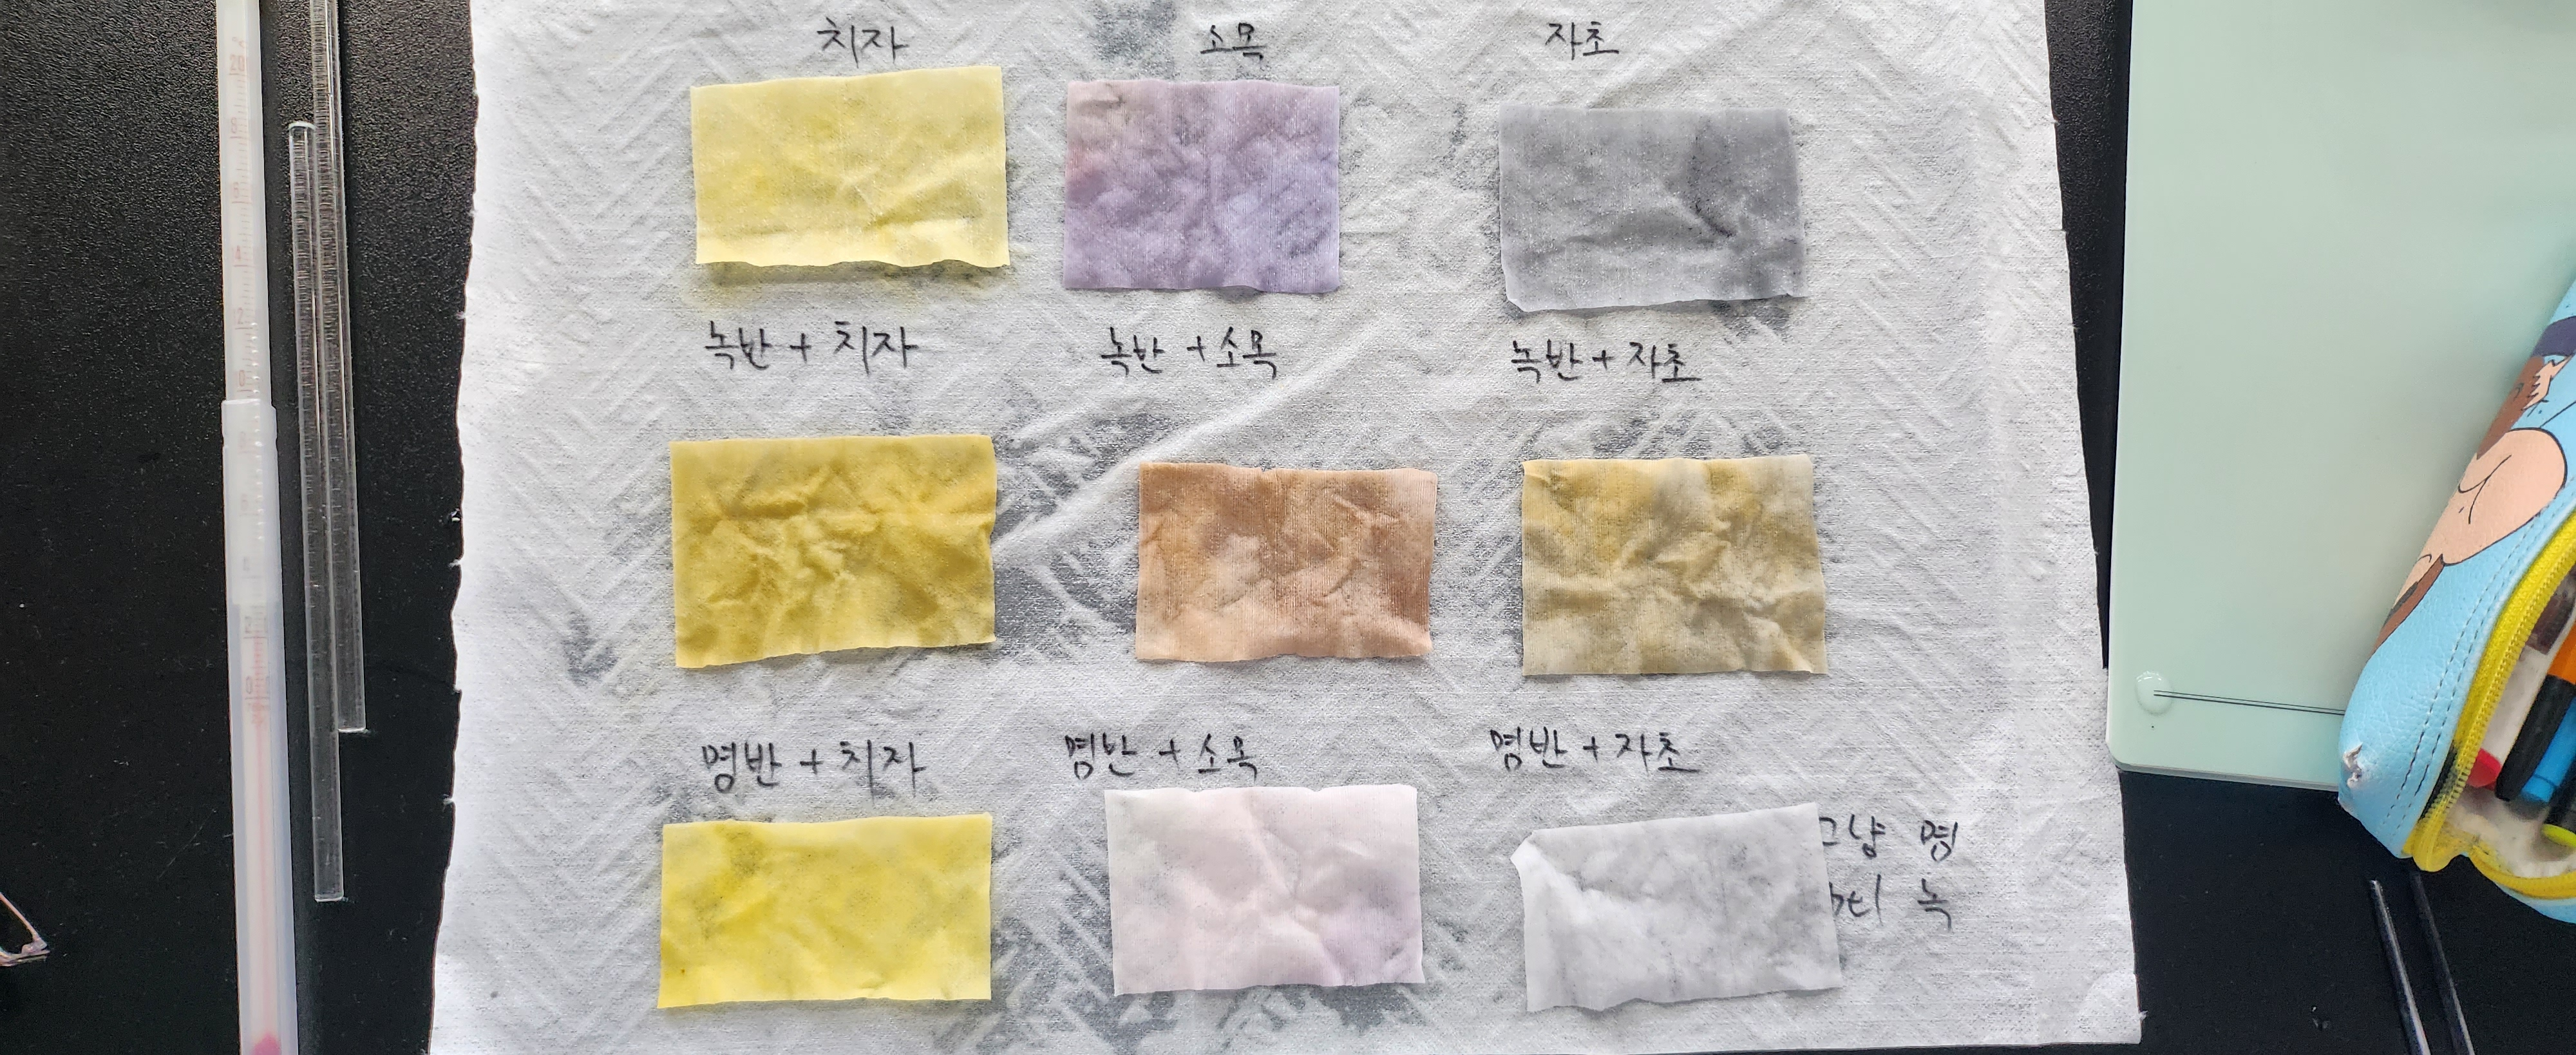
\includegraphics[width = 0.95\linewidth]{After.png}% Here is how to import EPS art
	\caption{\label{fig:After}반응 이후 결과}
\end{figure}

치자의 크로신 같은 경우 매우 길고 비대칭적인 분자구조를 가진다. 따라서 큰 dipole moment값을 가져 매염제 없이도 충분히 셀룰로우스, 혹은 polyamide와 강하게 결합할 수 있었을 것이다. 녹반, 명반과 같은 매염제가 추가된 이후에도 강한 극성을 띠어 금속원자와 강한 배위결합을 할 수 있게되어 색이 더 진해졌음을 알 수 있다. 이 때 크로신의 경우 $pH$에 변하더라도 전체 분자구조의 길이와 비교하여 공명하는 결합의 길이가 크게 변화하지 않는다. 따라서 아세트산, $NaHCO_{3}$과 반응하여도 색깔이 변하지 않으며 강한 배위결합으로 결합이 분리되지 않는다.\\

소목의 브라질레인의 경우 Fig.\ref{fig:Brazilein}에서 알 수 있듯 중성 pH에서는 강한 극성을 띤다. 하지만 pH가 증가함에 따라 Fig.\ref{fig:Brazilein}의 Form1 형태로 반응이 옮겨가면서 분자가 대칭적인 구조로 변하게 된다. 이로 인해 분자와 면섬유 사이의 결합력이 약해지게 되고 분자 전체길이와 비교한 공명 길이 또한 변화하므로 아세트산과 반응할 경우 색깔이 변화하게 된다. 하지만 $NaHCO_{3}$와 반응하는 경우 $NaHCO_{3}$의 $pKa=6.3$[7]가 아세트산의 $pKa=4.75$[2]보다 작아 반응성이 작아 큰 색깔 변화가 발생하지 않는다. 명반의 경우 $KAl(SO_{4})_{2}$의 $Al$이 $Fe$보다 반응성이 커 아세트산과 반응하여 색이 빠지게 된다. 하지만 $NaHCO_{3}$의 pKa가 작아 명반을 이용한 경우에도 소목은 반응하지 않는다. 녹반의 경우 $Fe$이 염료와 강하게 결합하여 산에 반응하지 않는다. \\

자초의 시코닌의 경우 하이드록시기가 대칭적으로 구성되어 면섬유와 잘 결합하지 않는다. 따라서 다른 염색된 면섬유들에 비해 색이 연하다. 하지만 주변의 분위기가 산성이 되는 경우 하이드록시기의 $OH$가 $O^{-}$가 되어 분자가 비대칭성이 커져 오히려 극성이 커지고 면섬유와의 결합이 강해진다. 녹반, 명반을 이용한 경우에도 마찬가지의 경향성을 보여 산염기에 의한 색변화를 거의 보여주지 않는다. \\

녹반을 이용하는 경우 면섬유가 대체로 노랑색에 가까워지는 경향성이 보인다. 또한 명반을 쓰는 경우 면섬유가 대체로 연해지는 경향성을 보인다. 이것은 전이금속의 $d-orbital$의 전자 전이로 인한 색깔에 해당한다. 

\section{\label{sec:level1}Conclusion}
천연염료를 이용한 염색의 경우 색깔이 잘 나타났으나 소목을 제외한 면섬유들의 경우 산용액에 크게 반응하지 않았다. 더 큰 $pKa$를 가지는 산용액을 이용할 경우 더 큰 색변화를 확인할 수 있을 것이며 이러한 예로 $HCl$, $H_{2}SO_{4}$와 같은 강산을 사용할 수 있을 것이다. 또한 본 실험의 결과는 대부분 하이드록시기에 의한 결과이다. 만약 염기 용액을 이용해 실험을 진행할 경우 다른 작용기에 의한 결과를 확인할 수 있을 것이다.

\section{\label{sec:level1}Reference}
[1] 김. (2016). 천연 색소의 추출과 무기 안료의 합성. In \textit{일반화학실험} (p. 158).

[2] Oxtoby, D., Gillis, H., \& Campion, A. (2007, April 2). Bonding in Transition Metal Compounds and Coordination Complexes. In \textit{Principles of Modern Chemistry} (6th ed., pp. 345–348, 634). Cengage Learning.

[3] Smith, J. (2010, January 8). Amines. In \textit{Organic Chemistry} (3rd ed., pp. 988–990). McGraw-Hill Education.

[4] Ngamwonglumlert, L., Devahastin, S., Chiewchan, N., \& Raghavan, G. S. V. (2020, July 24). Color and molecular structure alterations of brazilein extracted from Caesalpinia sappan L. under different pH and heating conditions. \textit{Scientific Reports, 10(1)}, 3. https://doi.org/10.1038/s41598-020-69189-3

[5] National Center for Biotechnology Information (2023). PubChem Compound Summary for CID 5281233, Crocin. Retrieved October 2, 2023 from https://pubchem.ncbi.nlm.nih.gov/compound/Crocin.

[6] Yadav, S., Sharma, A., Nayik, G. A., Cooper, R., Bhardwaj, G., Sohal, H. S., Mutreja, V., Kaur, R., Areche, F. O., AlOudat, M., Shaikh, A. M., Kovács, B., \& Mohamed Ahmed, A. E. (2022, July 1). Review of Shikonin and Derivatives: Isolation, Chemistry, Biosynthesis, Pharmacology and Toxicology. \textit{Frontiers in Pharmacology, 13}, 2. https://doi.org/10.3389/fphar.2022.905755

[7] National Center for Biotechnology Information (2023). PubChem Compound Summary for CID 516892, Sodium Bicarbonate. Retrieved October 2, 2023 from https://pubchem.ncbi.nlm.nih.gov/compound/Sodium-Bicarbonate.


\end{document}
%
% ****** End of file apssamp.tex ******
